\documentclass[12pt,a4paper]{scrartcl}
\usepackage[english]{babel}
\usepackage[T1]{fontenc}
\usepackage[utf8]{inputenc}
\usepackage[color=yellow!15]{todonotes}
\usepackage{graphicx}
\usepackage[numbers, sort&compress, square]{natbib}
\usepackage[colorlinks, linkcolor=black, citecolor=blue, urlcolor=blue]{hyperref}
\usepackage{titlesec}
\usepackage{color}
\usepackage{booktabs}

% used for line numbering
\usepackage{lineno}

\makeatletter
\renewcommand\section{\@startsection{section}{1}{\z@}%
                     {-7.5ex \@plus -1ex \@minus -10.2ex}%
                     {2.3ex \@plus.2ex}%
                     {\sffamily\large\bfseries}}
\makeatother


\usepackage{geometry}
\geometry{a4paper, top=35mm, left=30mm, right=30mm, bottom=35mm,
headsep=10mm, footskip=12mm}

\title{\textbf{ \Large {Reducing data traffic in wireless structural health monitoring systems using embedded computing}}}
\author
{\large Katrin Jahr, Robert Schlich\\
\\
\normalsize{Degree program “Civil Engineering” (M.Sc.)}\\
\normalsize{Bauhaus-Universität Weimar, Germany}\\
\\
\normalsize{katrin.jahr@uni-weimar.de \qquad}
\normalsize{robert.schlich@uni-weimar.de}
}
\date{}

\clubpenalty = 10000 % schliesst Schusterjungen aus
\widowpenalty = 10000 \displaywidowpenalty = 10000% schliesst Hurenkinder aus 

\newenvironment{sciabstract}{%
\begin{quote} \itshape}
{\end{quote}}

\begin{document} 

% Double-space the manuscript.

\baselineskip20pt

% Make the title.

\maketitle 
\vspace{-2em}

% 
%\sloppy
\setlength{\emergencystretch}{3pt}
\hyphenation{sample-rate auto-nomous moni-toring methods}


\begin{sciabstract}
Immense amounts of data incure during wireless structural health monitoring.
Applying adequate data compression methods can significantly reduce the amount of data that has to be transmitted and stored.
In this paper, the design and implementation of a wireless structural health monitoring system, capable of dezentralized data compression, is presented. 
A fast Fourier transform is embedded into each sensor node to analyze oscillation frequencies. 
By only transmitting the first natural frequency and the correlating magnitude, the data stream is reduced to two values per sampling event.
The proposed approach was validated in laboratory experiments.

\end{sciabstract}

%----------------------------------------------------------------------------------------

\section*{Introduction}

Civil engineering structures are exposed to various external impacts during their lifetime. 
Structural health monitoring (SHM) systems can be deployed to evaluate the conditions and to ensure the structural stability of civil engineering structures.
\citet{BisbySHM} defines SHM as "a non-destructive \textit{in-situ} structural evaluation method that uses any of several sensors which are attached to, or embedded in, a structure".
The obtained sensor data is collected by sensor nodes, and then analyzed and stored on a computer system over long periods of time. 
The analysis of the sensor data can reveal abnormal changes in material and geometric behaviour at an early stage.

Traditionally, the sensor nodes are connected to computer systems with cables.
Using wired SHM systems has several disadvantages, including expensive wiring, high installation and labor costs as well as inaccessibility of optimal sensor location with wires.
In wireless SHM systems, the sensor nodes communicate with each other and with computer systems via wireless transceivers, eradicating wiring-specific problems.

However, when using wireless SHM systems, special attention has to be paid to data transfer.
Immense amounts of raw data incure and have to be transmitted.
Over the air transmission is error-prone and may lead to data loss.
To save transmission time and storage space, and to decrease the probability data loss, the transmitted data can be reduced using embedded computing.
Depending on the measuring objective, first steps of data processing can be conducted decentralized directly on the sensor nodes.
Transmitting analysis results instead of raw data can reduce the amount of transmitted data exponentially.

In this paper, the natural frequency of a building structure is determined using a fast Fourier transform (FFT).
Deviations from the natural frequency indicate changes in the vibration behavior, which may be caused by structural failures.

This paper is organized as follows:
First, a wireless structural health monitoring system is designed and implemented. 
Next, a decentralized data analysis approach, using fast Fourier transform, is developed.
Then, the system is tested in laboratory experiments.
Finally, the experimental results are discussed and future research directions are proposed.

%----------------------------------------------------------------------------------------

\section*{Design and implementation of the wireless structural health monitoring system}
In the following section, the wireless structural health monitoring system is introduced and the software implementation is described.
The wireless SHM system consists of wireless sensor nodes and a host computer, linked with a basestation.
The sensor nodes and the basestation are of type "Oracle Sun SPOT". 
The Sun SPOTS are equipped with several components.
Among others, the sensor board includes an accelerometer and eight independent RGB-LEDs.
The 3-axis digital output accelerometer with sensitivity ranging between $\pm$\,2\,g and $\pm$\,8\,g has a maximum sampling rate of 125\,Hz \citep{eDemo2010}.

The SHM system performs the following tasks:
1. data acquisition,
2. data processing,
3. data transmission, 
4. data storage,
5. diagnostics and 
6. information retrieval.
The dataflow is illustrated in \autoref{fig:flow}.
Tasks 1 to 3 are executed by the sensor nodes: During system operation, the sensor nodes acquire acceleration measurements and perform a FFT to determine the characteristics of the oscillation of the structure. 
The processed data is then transmitted via radio to the basestation and, finally, to the host computer.
On the host computer, tasks 4 is conducted by storing the data in a MySQL database.
Task 5 and 6---additional analysis and diagnosis---are conducted on the host computer in further steps.

\begin{figure}[ht]
    \centering
    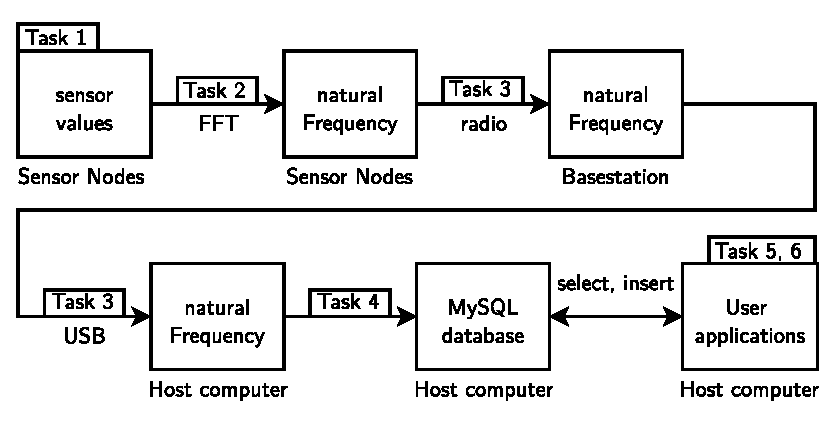
\includegraphics{figures/dataflow_tasks.eps}
    \caption{Dataflow and associated SHM tasks}
    \label{fig:flow}
\end{figure}

The SHM system is programmed object-oriented in Java. 
Object orientation uses objects, which are instanciated using classes as paradigm. 
A class includes methods, allowing the objects to perform actions, and attributes, storing object-specific data.
The SHM system consists of two packages---\texttt{sensornode} and \texttt{basestation}.
A package organizes several Java classes that build a program.

\autoref{fig:UML-sn} describes the classes of the \texttt{sensor\-node} package.
The package \texttt{sensor\-node} consists of the classes \texttt{Acceleration\-Sampler}, \texttt{FFT}, \texttt{Communi\-cation} and \texttt{Main\-Spot}, which are embedded directly into the sensor nodes.
The \texttt{Acceleration\-Sampler} class is responsible for measuring the acceleration.
There are two phases: At first, the acceleration is measured with a low sampling rate.
Once the acceleration exceeds a threshold, the second phase is entered by increasing the sampling rate. 
The measured values are stored into an array.
The different phases are indicatad by lighting different LEDs.
The \texttt{FFT} class performs a FFT on the measured accelerations. 
With the transformed data, the magnitudes and the correlating frequencies of the measured oscillation are calculated.
Finally, the natural frequency is determined by extracting the maximal magnitude.
The \texttt{Communi\-cation} class opens a radio connection between the sensor node and the basestation to transfer data from the sensor node to the basestation.
For starting the operation of the sensor node, the entry point of the programm is the \texttt{start\-App()} method in the \texttt{Main\-Spot} class. 
Within the \texttt{Main\-Spot} class, instances of the \texttt{Acceleration\-Sampler} class, the \texttt{FFT} class and the \texttt{Communication} class are created to perform the measurement.

\begin{figure}[ht]
    \centering
    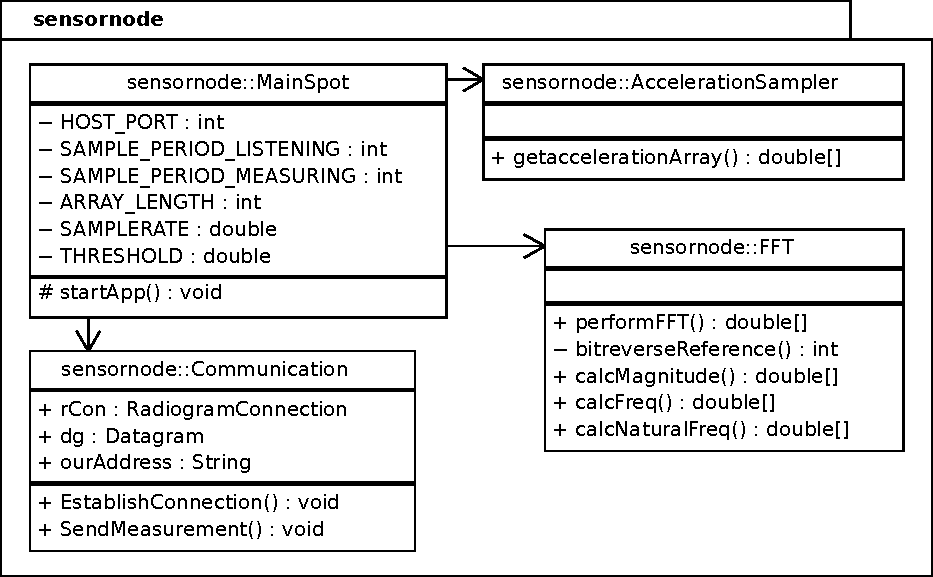
\includegraphics[width = \textwidth]{figures/uml-sensornode.pdf}
    \caption{Class diagram of the \texttt{sensornode} package}
    \label{fig:UML-sn}
\end{figure}

\autoref{fig:UML-bs} describes the classes of the \texttt{base\-station} package.
The package \texttt{base\-station} runs on the host computer and operates the basestation.
It consists of the classes \texttt{Database\-Handler} and \texttt{Main\-Base}.
The \texttt{Database\-Handler} class establishes a connection to a MySQL database, creates a database table, if none with the specified name is available, and inserts data into the database table.
The entry point of the program is the \texttt{run()} method in the \texttt{Main\-Base} class. The \texttt{Main\-Base} class opens a radio connection between the basestation and the sensor nodes, receives data sent by the sensor nodes and creates an instance of \texttt{Database\-Handler} to insert the data into the database.

\begin{figure}[h!]
    \centering
    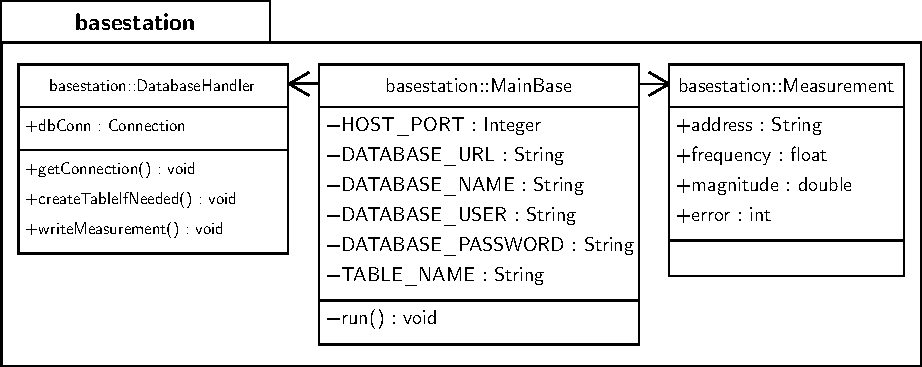
\includegraphics[width = \textwidth]{figures/uml-basestation.pdf}
    \caption{Class diagram of the \texttt{basestation} package}
    \label{fig:UML-bs}
\end{figure}

%\newpage

%----------------------------------------------------------------------------------------

\section*{Laboratory experiments}

In the following section, the laboratory experiments are described.
First, a description of the test setup is given, second, the data aquisition and processing are depicted, and finally, the results are discussed. 

To validate the proposed approach in laboratory experiments, the wireless SHM system is installed on a test structure.
The test structure is a 4-story shear-frame consisting of four steel plates of 25\,cm\,$\times$\,50\,cm\,$\times$\,0.8\,mm.
The plates are mounted on threaded rods with a vertical clearance of 23\,cm.
At the bottom, the rods are fixed into a solid block of 40\,cm\,$\times$\,60\,cm\,$\times$\,30\,cm.
The SHM system is installed on the test structure by fastening one wireless sensor node to each of the top three stories.
The laboratory setup is shown in \autoref{fig:teststructure}.

\begin{figure}[ht]
    \centering
    \includegraphics[scale=0.4]{figures/testsetup.png}
    \caption{Laboratory setup (Source: own photograph)}
    \label{fig:teststructure}
\end{figure}

The structure is excited by deflecting and releasing the top of the structure.
This excitation method ensures a free vibration in natural frequency with little interferences.
After excitation, when the acceleration threshold is exceeded, the sensor nodes automatically start measuring the acceleration.
To minimize the wireless data traffic, each sensor node performs a FFT, once sufficient acceleration measurements have been collected.
By the use of the FFT, the acceleration measurements are converted into the oscillation frequencies and the corresponding magnitudes of the building \cite{rao2011fast}.


The implementation of the FFT has been verified by plotting the frequency domain of various oscillation events, see \autoref{fig:76hzfft}.
The natural frequencies can be identified by the peaks in the magnitude graph.
The first two natural frequencies are located at approximately 2.3\,Hz (1\textsuperscript{st} natural frequency) and 8\,Hz (2\textsuperscript{nd} natural frequency).
Each sensor node transfers the values of the first natural frequency and the corresponding magnitude to the basestation. 
The values are stored in a MySQL database and analyzed.

\begin{figure}[htb]
    \centering
    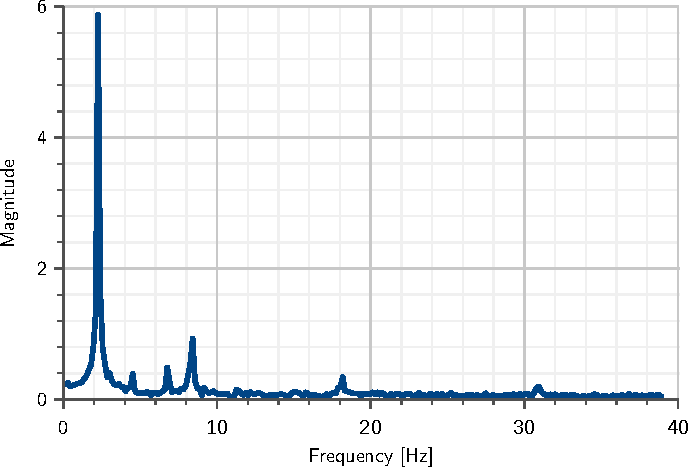
\includegraphics[scale=0.9]{figures/76HzHalf.pdf}
    \caption{frequency domain graph of the oscillation}
    \label{fig:76hzfft}
\end{figure}

The natural frequencies have been validated by repeated tests---using varying excitation forces, varying sampling rates, and varying quantities of measured values---and the results of a FE analysis.
The highest possible sampling rate was determined at 76\,Hz.
Higher samping rates could not be handled by the sensor nodes.
Test runs with more than 512 measured values showed no significant increase in precision.
Therefore, a sampling rate of 76\,Hz and 512 measured values were chosen.

Every sensor calculated the same natural frequency to a precision of four decimal points regardless of sensor position and degree of excitation.
Example results are shown in \autoref{tab:lab-ex}.
The identified magnitudes increase with ascending sensor node position from top to bottom, corresponding to the higher deflection at the top of the structure.

Through FFT analysis of sampling events, the data traffic is decreased from 512 doubles per sampling event to two doubles per sampling event.
A number stored in the used data format double occupies 8\,bytes of space.
The data traffic is decreased by (512$-$2)$\times$8\,B\,=\,4080\,B\,=\,3,98\,MB per sampling event, decreasing data traffic by 99.6\,\%.


\begin{table}[hb]
	\centering
	\begin{tabular}{l l c c c}
		\toprule
		ID & Position & Magnitude & Natural frequency [Hz] & Sampling rate [Hz]\\ 
		\midrule
		1 & top & 3.78 & 2.2461 & 76\\ 
		1 & middle & 3.23 & 2.2461 & 76\\ 
		1 & bottom & 1.97 & 2.2461 & 76\\ 
		\midrule	
		2 & top & 5.74 & 2.2536 & 76\\  
		2 & middle & 4.38 & 2.2536 & 76\\ 
		2 & bottom & 2.55 & 2.2536 & 76\\
		\midrule
		3 & top & 8.20 & 2.2536 & 76\\
		3 & middle & 6.35 & 2.2536 & 76\\ 
		3 & bottom & 3.79 & 2.2536 & 76\\
		\bottomrule
	\end{tabular}
	\caption{Natural frequencies of the test structure}
	\label{tab:lab-ex}
\end{table}

%----------------------------------------------------------------------------------------

\section*{Summary}

In structural health monitoring, a decentralized data compression strategy reduces data traffic and storage space.
Using a fast Fourier transform to determine the natural frequency allows conclusions about the structural integrity of a structure.
The transmitted data was reduced exponentially, saving up to 3,96\,MB per sampling event.

%----------------------------------------------------------------------------------------

\bibliographystyle{unsrtnat}
\bibliography{literature}

\end{document}
